% - machine learning e seleção de características
%    problema: falta de amostras
%    solução: simplificar o modelo de aprendizado -> seleção de 
%             características    
% - problema de otimização
% - funções de custo
% - aplicações: w-operadores, construção de modelos funcionais
% - algoritmos de seleção de características
% - trabalhos antigos

Seleção de características é uma técnica que pode ser utilizada em uma 
das etapas da construção de um modelo de aprendizado de máquina. Ela 
consiste em, dado o conjunto de características observadas nas amostras,
escolher um subconjunto que seja ótimo de acordo com alguma métrica. 
Devemos considerar o uso de seleção de características quando a 
quantidade de características é muito grande, o que pode tornar o uso do
modelo muito caro do ponto de vista computacional. Outra aplicação dessa 
técnica é em situações nas quais a quantidade de amostras é pequena 
comparada à complexidade do modelo original, em outras palavras, quando 
ocorre sobreajuste (do inglês, \foreignword{overfitting}).

Mais formalmente, o problema de seleção de características consiste em
um problema de otimização combinatória em que, dado um conjunto $S$ de 
características, procuramos por um subconjunto $X \in \powerset (S)$
ótimo de acordo com uma função de custo $c : \mathcal{P}(S) \to 
\fieldR_{+}$. É comum nas abordagens do problema explorar o
fato de que o espaço de busca $\powerset(S)$ junto a relação $\subseteq$
define um reticulado Booleano~\cite{Rei12,AG+18}. No geral, a 
função de custo $c$ deve ser capaz de medir quão informativas as 
características $X$ são em respeito ao rótulo $Y$ do problema de 
aprendizado; portanto $c$ costuma depender da estimação da distribuição 
de probabilidade conjunta de $(X, Y)$.

Quando ocorre a estimação da distribuição de probabilidade conjunta de 
$(X, Y)$, o custo das cadeias do reticulado Booleano reproduzem um
fenômeno conhecido em aprendizado de máquina, o das ``curvas em U''. 
Para entender intuitivamente esse fenômeno, devemos observar que 
conforme subimos uma cadeia do reticulado estamos aumentando o número de
características sendo consideradas, portanto existem mais possíveis
valores de $X$, permitindo descrever melhor os valores de $Y$; por outro
lado, também precisaríamos de mais amostras para estimar bem 
$\probability (X, Y)$, e, quando isso não é possível, erros de estimação
fazem com que $c(X)$, isto é, o custo de $X$, aumente.

Podemos então considerar um caso particular do problema de seleção de
características em que a função de custo descreve ``curvas em U''
em todas as cadeias do reticulado Booleano. Esse caso particular é 
conhecido como problema U-curve e existem na literatura algoritmos 
ótimos para esse problema como o \algname {U-Curve Branch and Bound 
(UBB), U-Curve-Search (UCS) e Poset Forest Search (PFS)}~\cite{RFB14,Rei12}. A solução do problema 
U-curve tem aplicações em problemas de aprendizado de máquina tais como 
como projeto de W-operadores~\cite{MJCJJB} e preditores na estimação de 
Redes Gênicas Probabilísticas~\cite{BCJMJ07}.

\begin{figure}[ht]
    \centering
    \begin{tabular}{c c}
    \subfigure[] {\scalebox{.75}{
        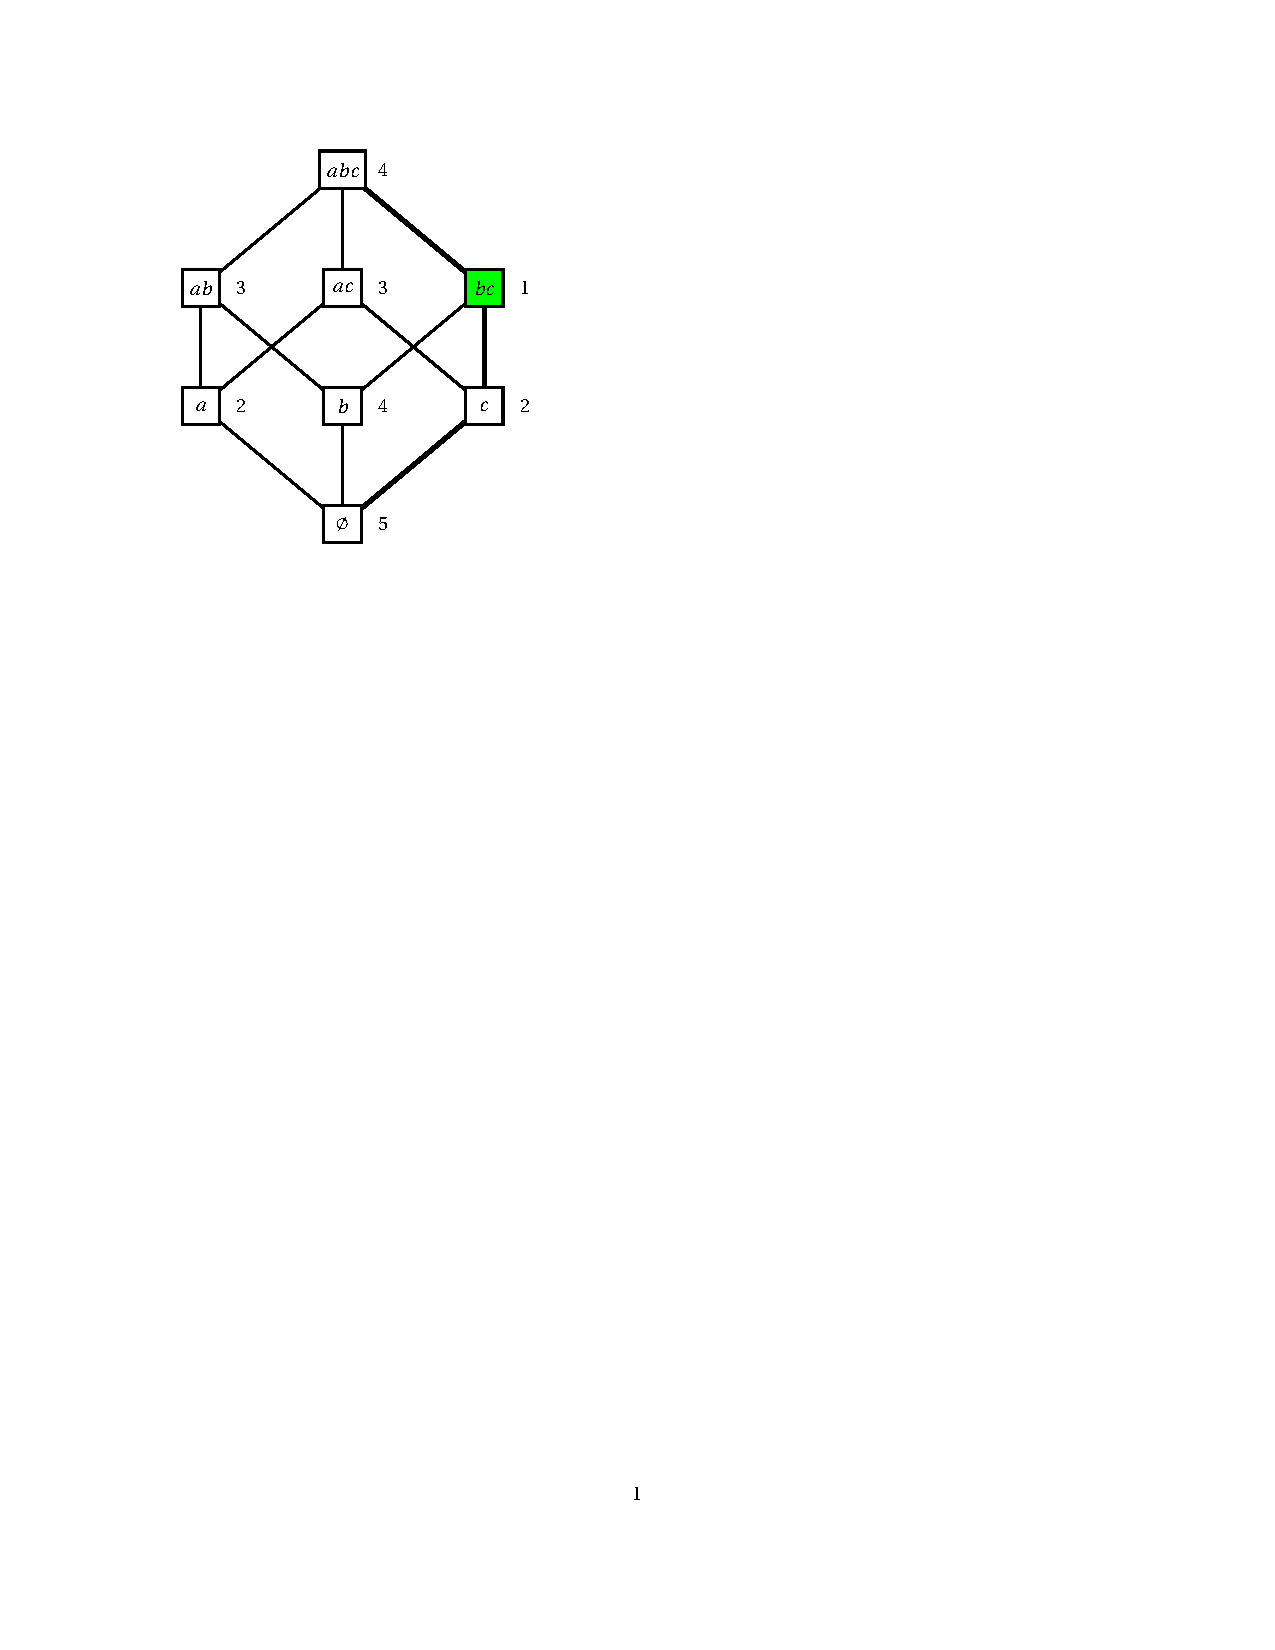
\includegraphics[clip=true, trim={3cm 18cm 13cm 2cm}]{intro/example_lattice_3.pdf}}
    \label{fig:intro:lattice} }
    & 
    \subfigure[] {\scalebox{.3}{
        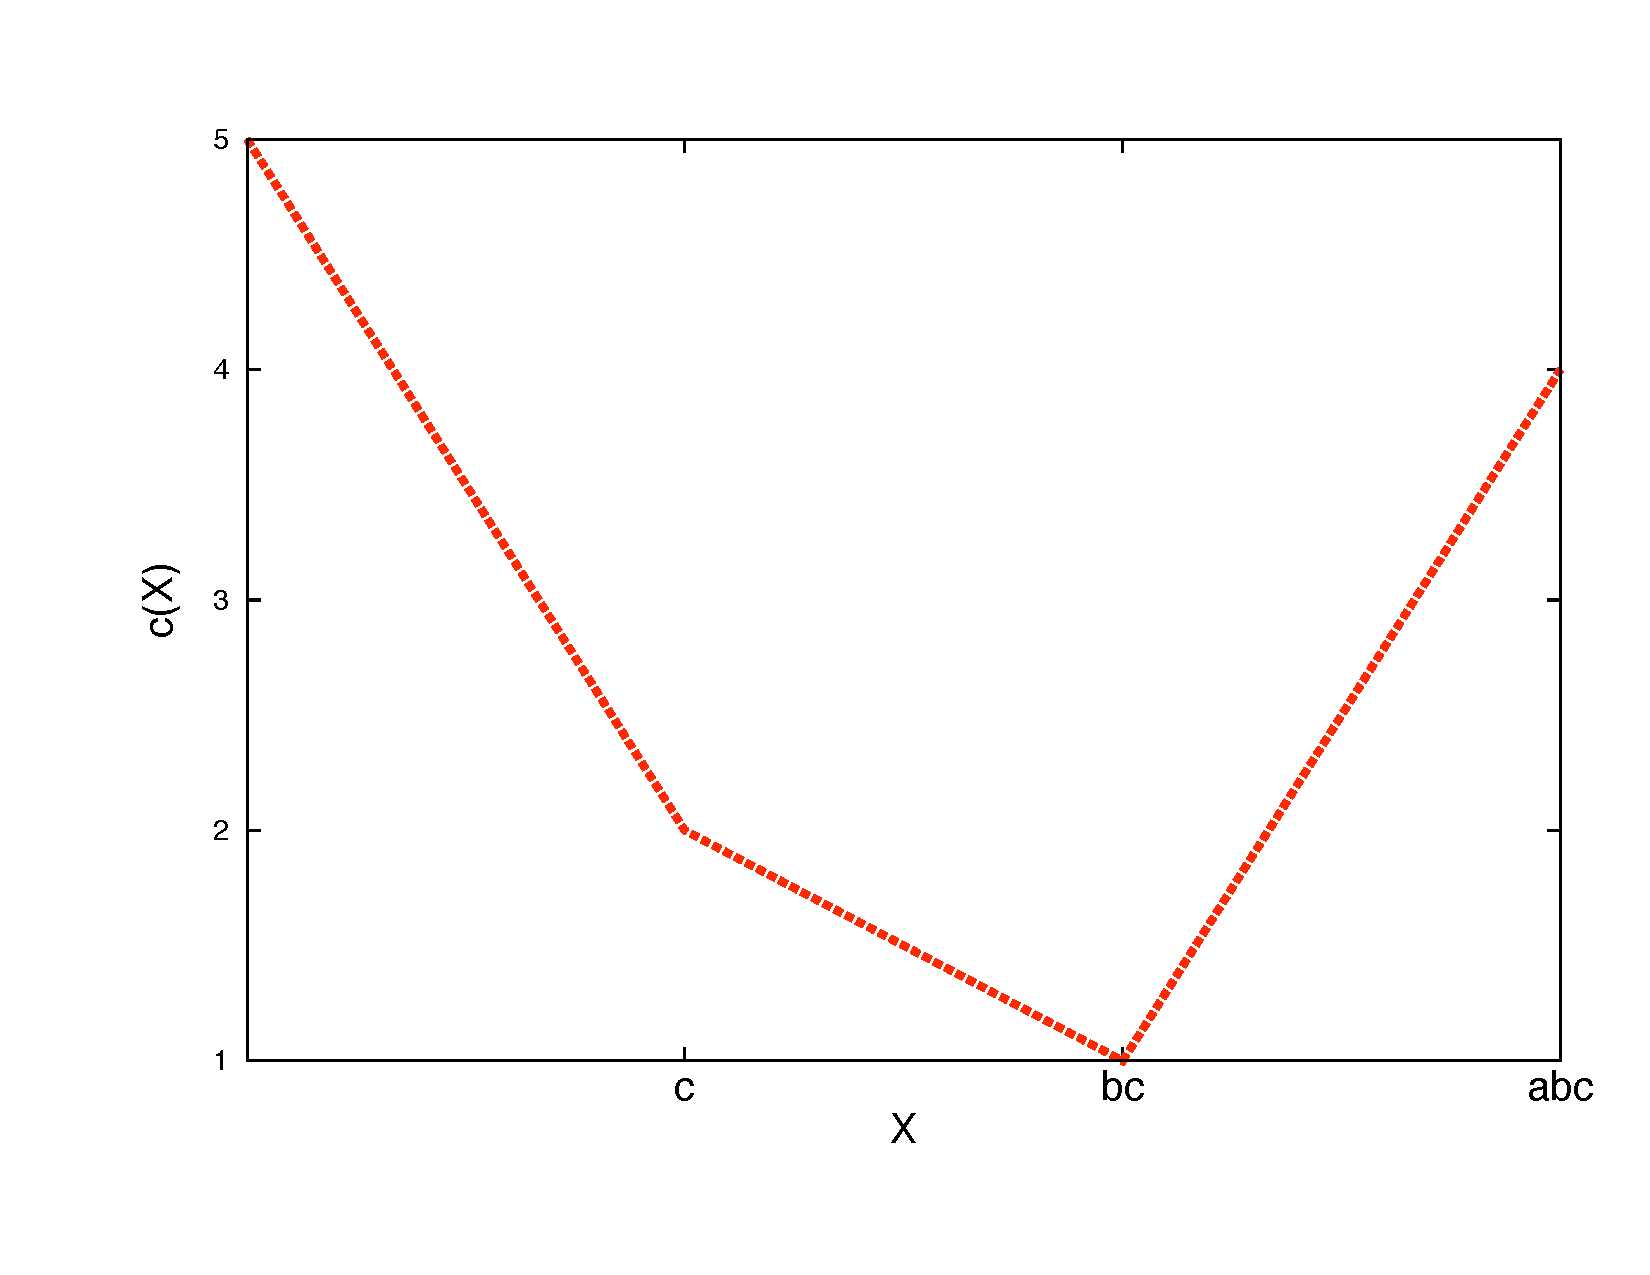
\includegraphics[clip=true, trim={1cm 0cm 1cm 2cm}]{intro/example_lattice_chain_3.pdf}}
    \label{fig:intro:chain} }
    \end{tabular}
    \caption{Exemplo de instância do problema U-curve em que o conjunto 
    de características é $S = \{a, b, c\}$. A figura 
    \ref{fig:intro:lattice} representa o diagrama de Hasse do reticulado 
    Booleano $(\powerset (S), \subseteq)$, anotando ao lado de cada 
    conjunto de características o seu custo. Os custos dos elementos da 
    cadeia $\{\emptyset, c, bc, abc\}$, marcada em negrito, são 
    apresentados na figura \ref{fig:intro:chain}. O subconjunto 
    $\{b,c\}$, marcado em verde, tem custo mínimo na cadeia em negrito 
    e também no reticulado inteiro e, portanto é a solução ótima para 
    esta instância. Imagem retirada de ~\cite{Rei12} com permissão do 
    autor.}
\end{figure}

O problema U-Curve é NP-difícil~\cite{Rei12}; por conta deste fato, os 
algoritmos apresentados até então na literatura têm limitações tanto do 
ponto de vista de tempo de computação quanto do uso de memória. Dentre 
estes algoritmos, destacamos o PFS, que foi criado como um melhoramento 
do algoritmo UBB. 

O \algname{UBB} é um algoritmo \foreignword{branch-and-bound} que, a 
partir de uma enumeração, representa o espaço de busca como uma árvore 
e procura pelo mínimo global fazendo uma espécie de busca em 
profundidade que percorre as cadeias da árvore do espaço de busca, 
podando nós (e consequentemente seus descendentes) sempre que a função 
de custo cresce. Este algoritmo é unidirecional no sentido de que a 
busca em profundidade percorre as cadeias da árvore de baixo para cima, 
portanto se o custo dos elementos de uma cadeia nunca crescem então 
todos elementos desta serão visitados. A limitação deste algoritmo é 
evidente quando a função de custo usada é monótona não-crescente, 
pois isto implica que a condição de poda nunca será verdadeira, fazendo 
com que todo o espaço de busca seja percorrido.

O algoritmo \algname{PFS} contorna esta limitação porque é bidirecional.
Para fazer isto, ele precisa representar o espaço de busca de duas 
maneiras diferentes: uma que é similar ao que o \algname{UBB} faz, para
os percorrimentos de baixo para cima, e outra que deve ser uma 
representação equivalente a primeira para o reticulado Booleano dual 
$(\mathcal{P}(S), \supseteq)$, para os percorrimentos de cima para 
baixo; ambas representações são feitas com florestas de posets, em uma
estrutura de dados capaz de armazenar raízes e adjacências dos nós. Uma
iteração do \algname{PFS} é constituída das seguintes etapas: escolha de
uma direção de percorrimento; escolha de uma raíz na floresta escolhida;
ramificação (percorrimento de uma cadeia); poda na floresta escolhida; 
e por último, atualização da floresta dual a escolhida para que ambas
representem o mesmo espaço de busca.

Existem pontos do algoritmo \algname{PFS} que ainda não foram explorados
com o intuito de melhorar seu desempenho. Dentre eles, a escolha de 
raízes para etapa de ramificação, que é feita de maneira arbitrária 
atualmente; o uso de outras estruturas de dados para representação das 
florestas, como por exemplo diagramas de decisão binárias ordenados 
(\foreignword{Ordered Binary Decision Diagrams} - OBDDs) ~\cite{Bry86}; 
e também a paralelização do código, o que parece trazer ganhos no tempo 
de execução do algoritmo dado que, como as árvores do espaço de
busca são disjuntas, a etapa de ramificação pode ser realizada de 
maneira paralela com pouca informação compartilhada entre threads.

% TODO:
%{\color{blue}[Comentário: acho que vai ter que revisar a explicação básica da dinâmica do PFS, detalhando-a mais e/ou fazendo referências para minha tese. Uma ideia seria aproveitar o que escrevemos sobre o PFS no projeto de mestrado]}.

\section{Objetivos do Trabalho}
Podemos dividir os objetivos deste trabalho em objetivos gerais e 
específicos.\\

{\bf Objetivos gerais}:
\begin{enumerate}
\item{Criar algoritmos para o problema U-curve que sejam mais eficientes
em consumo de tempo e/ou de memória do que as presentes soluções;}
\item{Verificar a qualidade das soluções encontradas no desenvolvimento
de modelos de Aprendizado Computacional.}
\end{enumerate}

{\bf Objetivos específicos}:
\begin{itemize}
\item{Estudar o algoritmo \algname {Poset Forest Search (PFS)};}
\item{Modificar a etapa de ramificação do algoritmo \algname{PFS} e 
    avaliar as mudanças na dinâmica do algoritmo;}
\item{Paralelizar o algoritmo \algname{PFS}, com as modificações feitas
    na etapa de ramificação (se houver melhorias com tal mudança);}
\item{Criar um novo algoritmo, de natureza paralela e facilmente 
    combinável com outros algoritmos, para o problema U-Curve (o 
    algoritmo \algname{PUCS});}
\item{Avaliar o consumo de recursos computacionais dos algoritmos 
    criados, comparando com os algoritmos já presentes na literatura 
    como o \algname{UBB};}
\item{Avaliar os conjuntos de características selecionados por cada 
    algoritmo na seleção de modelos de aprendizado computacional, usando 
    como exemplo conjuntos de dados do repositório 
    \href{https://archive.ics.uci.edu/ml/index.php}
        {UCI Machine Learning Repository.}}
\end{itemize}

\section{Organização do Trabalho}

A fazer, resumo de cada capítulo da monografia.

